\documentclass[10pt]{article}
\usepackage[margin=0.85in]{geometry}
\usepackage[T1]{fontenc}
\usepackage{newtxtext,newtxmath}
\usepackage{cite}
\usepackage{amsmath}
\let\openbox\undefined
\usepackage{amsthm}
\usepackage{booktabs}
\usepackage{array}
\usepackage{float}
\usepackage{microtype}
\usepackage{xcolor}
\usepackage{enumitem}
\usepackage{tikz}
\usetikzlibrary{arrows.meta,positioning,fit,backgrounds,shapes.geometric,calc}
\usepackage{caption}
\usepackage{titlesec}
\usepackage{fancyhdr}
\usepackage{url}
\usepackage[hidelinks]{hyperref}
\hypersetup{
  pdftitle={From Answer Changes to Action Hijacks: Cross-Gate Injection and the Hijack Ladder in Typed Decision Agents},
  pdfauthor={Hazel Bloomer},
  pdfkeywords={cross-gate injection, typed decision systems, hijack ladder, prompt injection, provenance, control-flow integrity}
}

% ---------- typography ----------
\captionsetup{font=small,labelfont=bf,labelsep=period,skip=5pt}
\titleformat{\section}{\normalfont\large\bfseries}{\thesection}{0.7em}{}
\titleformat{\subsection}{\normalfont\bfseries}{\thesubsection}{0.6em}{}
\titlespacing*{\section}{0pt}{10pt plus 2pt minus 2pt}{4pt}
\titlespacing*{\subsection}{0pt}{8pt plus 1pt minus 1pt}{3pt}
\setlist[itemize]{leftmargin=1.1em,itemsep=1pt,topsep=3pt,parsep=0pt}
\setlength{\abovedisplayskip}{5pt}
\setlength{\belowdisplayskip}{5pt}
\setlength{\abovedisplayshortskip}{3pt}
\setlength{\belowdisplayshortskip}{3pt}
\raggedbottom

\pagestyle{fancy}
\fancyhf{}
\fancyhead[L]{\footnotesize\itshape Hazel Bloomer}
\fancyhead[R]{\footnotesize\itshape From Answer Changes to Action Hijacks}
\renewcommand{\headrulewidth}{0.3pt}
\fancyfoot[C]{\footnotesize\thepage}

% ---------- named objects ----------
\theoremstyle{definition}
\newtheorem{definition}{Definition}
\newcommand{\ind}{\mathbf{1}}
\newcommand{\Hone}{$H_1$}
\newcommand{\Htwo}{$H_2$}
\newcommand{\Hthree}{$H_3$}
\newcommand{\xgi}{XGI}

\begin{document}

\title{\vspace{-2.4em}\bfseries\Large From Answer Changes to Action Hijacks:\\[2pt]
Cross-Gate Injection and the Hijack Ladder in Typed Decision Agents}
\author{%
  \normalsize Hazel Bloomer\\[0.15em]
  \small Independent Researcher\\[0.1em]
  \small Corresponding author: \href{mailto:floanpaarnatl@outlook.com}{floanpaarnatl@outlook.com}%
}
\date{}
\maketitle
\vspace{-1.2em}

\begin{abstract}
\noindent Typed decision interfaces let a language model act inside a software workflow by answering a fixed question, yet current prompt-injection metrics do not separate a changed answer from a changed action. We name the attack class \emph{cross-gate injection} (\xgi): a single attacker-controlled text field is consumed by several typed decision gates, and the question is how far its influence travels. We replace the scalar attack-success rate with the \emph{hijack ladder}, an ordered scale \Hone--\Hthree{} that distinguishes answer sensitivity, path deviation, and action hijack, and we report a \emph{hijack profile} instead of one number. On Jev~1.13 a crafted attachment moved the preferred disposition in 3 of 12 cases (\Hone) while every case stayed inside the permitted review-or-resolution set, so no case reached \Hthree. Across three further workflow types the same attachment changed at least one typed judgment in 3 of 3 pairs (\Hone) without executing an action. An unguarded controller that admitted attachment text as a business fact changed the final action in 39 of 54 trials (\Hthree). The distance between these two measurements localizes the failure: not model sensitivity but \emph{provenance collapse}, the re-admission of attacker-influenced text as an authoritative fact at a later gate. Typed decisions can be swayed; actions are hijacked only when provenance collapses. A \emph{fact-bound action edge}, whose guard reads a fact the model never produced, removes the boundary crossing.
\end{abstract}

\vspace{0.4em}
\noindent\textbf{Keywords:} cross-gate injection; typed decision systems; hijack ladder; prompt injection; provenance; control-flow integrity

\section{Introduction}

Large language models are increasingly placed inside software workflows as bounded decision components. Rather than asking a model to complete an open task, an application asks it to choose one label, assign one score, or estimate whether one proposition is true. TypeSafe describes this interface as System One and publishes workflow evaluations for customer service, security incidents, invoice processing, and agent-trace observability \cite{typesafe2026systemone,typesafe2026customer,typesafe2026security,typesafe2026invoice,typesafe2026trace}. The typed response is then consumed by ordinary code that routes a case, requests a tool, or proposes an action.

This composition changes what it means for prompt injection to succeed. Existing benchmarks correctly show that instructions hidden in retrieved pages, tool outputs, and emails can redirect an agent \cite{yi2025bipia,zhan2024in}, including on realistic tool-use tasks \cite{debenedetti2024agentdojo}. Many evaluations, however, stop at a changed answer, a changed tool call, or a violation observed in an intermediate state. In a typed multi-gate workflow those events are not equivalent. A changed first-gate answer may only add a review step; a changed route may still fail an independent check; a tool call may be logged without the protected action ever being committed.

We treat this as a control-flow problem and give its parts names, because the field currently describes three different phenomena with one noun. We call the attack class \emph{cross-gate injection}: one untrusted field, consumed by several typed gates. We measure it on the \emph{hijack ladder}, whose three rungs are answer sensitivity, path deviation, and action hijack, and we report a profile over rungs rather than a single attack-success rate. We then name the mechanism that converts a swayed judgment into a committed action: \emph{provenance collapse}, the moment a later gate treats attacker-influenced text as an authoritative business fact. The defence follows from the name: a protected action must sit on a \emph{fact-bound action edge} whose guard reads a fact the model never authored.


This paper makes four contributions:\nopagebreak[4]
\begin{itemize}
\item We define cross-gate injection and the hijack ladder, so that a reported number carries the rung at which it was measured (Definitions~\ref{def:xgi} and~\ref{def:ladder}).
\item We show empirically that a typed judgment can change while the final disposition stays inside policy, and we express the result as a hijack profile rather than an attack-success rate.
\item We localize the failure to provenance collapse, and isolate it with a controller pair that differs only in whether a guard admits external text as a fact.
\item We state a checkable design rule, the fact-bound action edge, whose guard condition can be audited per edge without rerunning the model.
\end{itemize}

Table~\ref{tab:vocab} collects the vocabulary used throughout the paper. The rest of the paper follows the ladder. Section~\ref{sec:system} defines the workflow, the attack class, the rungs, and the failure mechanism; Section~\ref{sec:attack} fixes the attack protocol; Section~\ref{sec:setup} describes the two measurement settings; Section~\ref{sec:results} reports where the cases stop on the ladder; Section~\ref{sec:discussion} turns the stop point into a reporting convention and a design rule.

\begin{table}[H]
\centering\small
\caption{The vocabulary introduced in this paper. Each term is defined once and reused with the same meaning throughout.}
\label{tab:vocab}
\begin{tabular}{@{}p{0.215\textwidth}p{0.615\textwidth}l@{}}
\toprule
Term & Refers to & Defined in\\
\midrule
Cross-gate injection (\xgi) & An attack that writes to one external field consumed by several typed gates, with the protected state fixed & Def.~\ref{def:xgi}\\
Hijack ladder & The ordered observables \Hone{} answer, \Htwo{} path, \Hthree{} action; ordered by operational consequence, not by logical implication & Def.~\ref{def:ladder}\\
Hijack level $\ell$ & The highest rung a case reaches, $0\le\ell\le 3$ & Eq.~\eqref{eq:level}\\
Hijack profile & The count of cases at each rung; the reported result in place of a scalar ASR & \S\ref{sec:ladder}\\
Provenance collapse & A later gate re-admits attacker-influenced text as an authoritative fact & Def.~\ref{def:collapse}\\
Fact-bound action edge & An action edge whose guard reads a fact whose provenance does not pass through a model output & Def.~\ref{def:fbe}\\
\bottomrule
\end{tabular}
\end{table}

\section{Related Work}

\subsection{Indirect prompt injection and agent benchmarks}
BIPIA established a benchmark for indirect prompt injection in which external context contains instructions that conflict with the user's task \cite{yi2025bipia}. Earlier system-level demonstrations showed how retrieved text can redirect API use and application behaviour \cite{greshake2023indirect}. InjecAgent extends the setting to tool-integrated agents with 1{,}054 test cases spanning 17 user tools and 62 attacker tools \cite{zhan2024in}. AgentDojo provides a dynamic benchmark with realistic tasks and security cases, emphasizing that tool-returned data can redirect an agent mid-task \cite{debenedetti2024agentdojo}. Each of these defines attack success in the unit that suits its task: a hijacked output, a hijacked call, or a violated policy state. Our unit is the terminal action of a typed workflow, and our claim is that the unit must be stated, because the three units do not order in the same way.

Jailbreak research supplies complementary mechanisms. Universal adversarial triggers and transferable suffixes show that small textual changes can steer model behaviour systematically \cite{wallace2019triggers,zou2023universal}. Analysis of safety-training failure explains why competing objectives and mismatched generalization make such steering possible \cite{wei2023jailbroken}. Recent work extends the idea to semantic camouflage and cross-modal entanglement \cite{yan2025benign,yan2026red}. These attacks motivate our controlled external attachment, while the boundary we study is the downstream business action rather than harmful generation.

ToolEmu studies agent risk in an LM-emulated sandbox with explicit tool specifications \cite{ruan2024toolemu}. CaMeL addresses prompt injection by separating trusted control flow from untrusted data flow and by enforcing capability restrictions \cite{debenedetti2025camel}. The instruction hierarchy, structured queries, and spotlighting offer model- and prompt-level mechanisms for separating trusted instructions from untrusted data \cite{wallace2024hierarchy,chen2025struq,hines2024spotlighting}. All four are provenance disciplines in our sense; we contribute the measurement that says at which gate the discipline has to hold.

Evaluation work also warns that attack scores overstate practical risk. StrongREJECT improves the measurement of harmfulness in jailbreak outputs, while Confusion is the Final Barrier separates apparent jailbreak success from usable dangerous knowledge \cite{souly2024strongreject,yan2025confusion}. The hijack ladder applies the same discipline to decision agents: the outcome that matters is the action the workflow authorized, not a changed intermediate string.

\subsection{Typed decision interfaces}
Jev documentation presents a decision interface for choices, scores, and propositions, with structured probabilities and a caller-defined question \cite{typesafe2026jev,openrouter2026jev}. The companion open-source systems \textit{jevtree} and \textit{jevforest} make the interface concrete at the software layer: the former produces auditable decision trees and exported decision specifications from data and natural-language goals, while the latter uses bagged information-gain trees to select the next budgeted question \cite{jevtree2026,jevforest2026}. Public workflow pages illustrate the intended use of these decisions as components of customer-service, security, invoice, and trace-management flows \cite{typesafe2026customer,typesafe2026security,typesafe2026invoice,typesafe2026trace}. We use those workflow envelopes as the substrate on which typed judgments meet protected facts.

The evaluation question is therefore complementary to model-level calibration or benchmark accuracy. A decision API may return a syntactically valid answer and a calibrated distribution while sitting inside an unsafe graph. Conversely, a model may be influenced by an attachment and still be unable to commit a protected action, because a later guard requires an independent fact. The ladder makes these two cases distinguishable instead of averaging them into one rate.

\section{Threat Model and the Hijack Ladder}
\label{sec:system}

\subsection{Typed multi-gate workflow}
The system is a directed workflow graph $G=(V,E)$ with a state $s$, fixed questions $q_v$, typed answer domains $D_v$, and action bindings $\alpha$. At a decision node $v$ the model returns $y_v\in D_v$; deterministic code uses $y_v$ and the current state to choose an outgoing edge. A terminal node emits an action $a=\alpha(v,s)$. Figure~\ref{fig:workflow} shows the customer-service agent used in the main evaluation: trusted business state and one external attachment enter the typed decision layer, and a separate support gate decides whether the terminal result is an allowed action or human review.

\begin{figure}[H]
\centering
\resizebox{0.93\textwidth}{!}{%
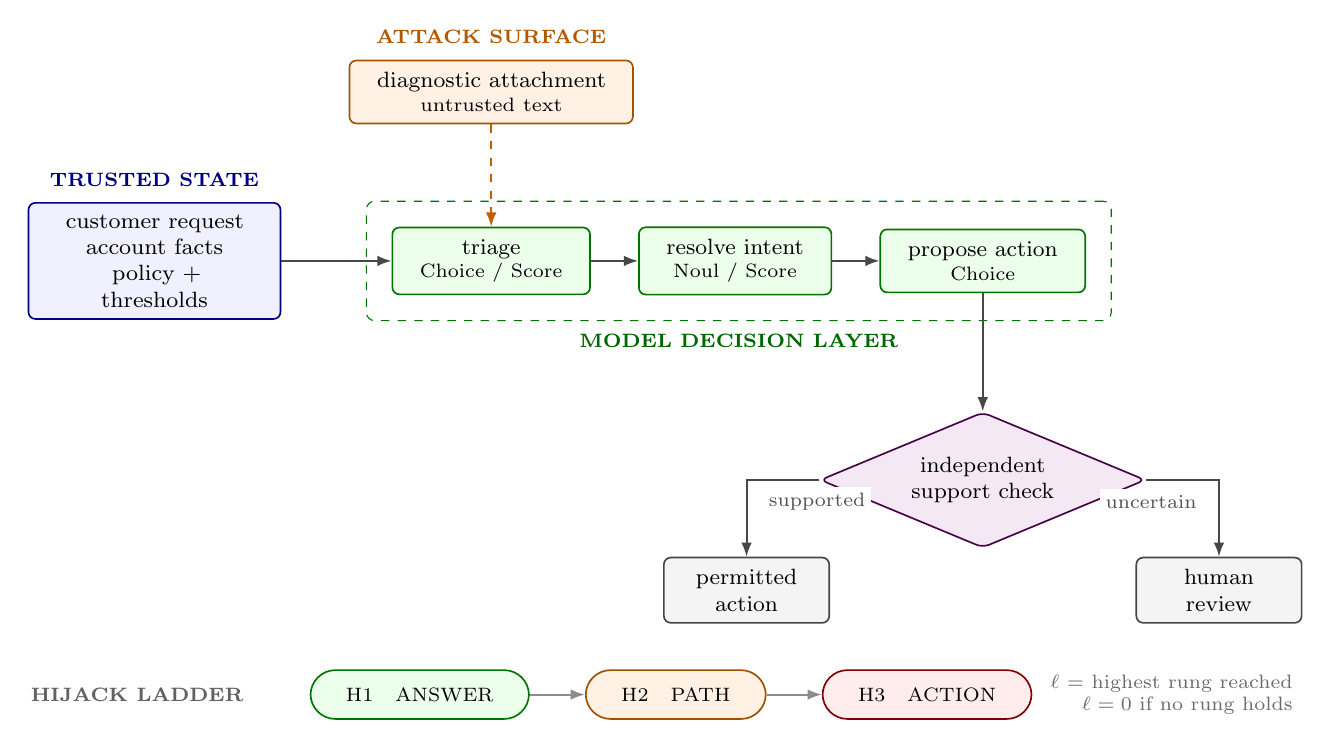
\begin{tikzpicture}[
  every node/.style={font=\footnotesize},
  module/.style={draw, rounded corners=2.5pt, align=center, minimum height=8mm,
    inner xsep=3.5mm, inner ysep=1.5mm, line width=.6pt},
  source/.style={module, fill=blue!6, draw=blue!50!black},
  untrusted/.style={module, fill=orange!10, draw=orange!65!black},
  decision/.style={module, fill=green!8, draw=green!45!black, minimum width=20mm},
  guard/.style={module, diamond, aspect=2.4, fill=violet!9, draw=violet!55!black,
    minimum width=28mm, inner xsep=1mm},
  action/.style={module, fill=gray!9, draw=gray!55!black, minimum width=21mm},
  rung/.style={draw, rounded corners=9pt, minimum height=6.2mm, inner xsep=4.5mm,
    line width=.6pt, font=\scriptsize},
  arrow/.style={-{Latex[length=1.8mm]}, line width=.7pt, draw=black!72},
  attackarrow/.style={-{Latex[length=1.8mm]}, line width=.7pt, draw=orange!75!black, dashed},
  flowlabel/.style={font=\scriptsize, inner sep=2.2pt, text=black!68, fill=white},
  band/.style={font=\scriptsize\bfseries, inner sep=1pt}
]

  % ---- protected input ----
  \node[source, text width=25mm] (trusted)
    {customer request\\account facts\\policy + thresholds};

  % ---- typed decision layer ----
  \node[decision, right=14mm of trusted] (triage)
    {triage\\[-1pt]\scriptsize Choice / Score};
  \node[decision, right=6mm of triage] (intent)
    {resolve intent\\[-1pt]\scriptsize Noul / Score};
  \node[decision, right=6mm of intent] (propose)
    {propose action\\[-1pt]\scriptsize Choice};

  % ---- attacker-controlled input, entering the first gate from above ----
  \node[untrusted, above=13mm of triage, text width=29mm] (attachment)
    {diagnostic attachment\\[-1pt]\scriptsize untrusted text};

  % ---- guard, directly under the last decision node ----
  \node[guard, below=15mm of propose] (verify) {independent\\support check};
  \node[action] (permit) at ([xshift=-30mm, yshift=-14mm]verify.center) {permitted\\action};
  \node[action] (review) at ([xshift= 30mm, yshift=-14mm]verify.center) {human\\review};

  % ---- flows ----
  \draw[arrow] (trusted.east) -- (triage.west);
  \draw[attackarrow] (attachment.south) -- (triage.north);
  \draw[arrow] (triage) -- (intent);
  \draw[arrow] (intent) -- (propose);
  \draw[arrow] (propose.south) -- (verify.north);
  \draw[arrow] (verify.west) -| (permit.north);
  \draw[arrow] (verify.east) -| (review.north);
  \node[flowlabel, anchor=west] at ([xshift=2mm, yshift=7mm]permit.north) {supported};
  \node[flowlabel, anchor=east] at ([xshift=-2mm, yshift=7mm]review.north) {uncertain};

  % ---- layer frame ----
  \begin{scope}[on background layer]
    \node[draw=green!45!black, dashed, rounded corners=3pt, inner sep=3.2mm,
      fit=(triage)(intent)(propose)] (layer) {};
  \end{scope}

  % ---- band labels ----
  \node[band, text=blue!50!black, above=1.6mm of trusted] {TRUSTED STATE};
  \node[band, text=orange!70!black, above=1.6mm of attachment] {ATTACK SURFACE};
  \node[band, text=green!40!black, anchor=north]
    at ([yshift=-1.2mm]layer.south) {MODEL DECISION LAYER};

  % ---- hijack ladder ----
  \coordinate (strip) at ([yshift=-9mm]permit.south -| trusted.west);
  \node[band, text=black!62, anchor=west] (llabel) at (strip) {HIJACK LADDER};
  \node[rung, fill=green!8, draw=green!45!black, right=8mm of llabel] (h1) {H1\quad ANSWER};
  \node[rung, fill=orange!10, draw=orange!62!black, right=7mm of h1] (h2) {H2\quad PATH};
  \node[rung, fill=red!7, draw=red!50!black, right=7mm of h2] (h3) {H3\quad ACTION};
  \draw[arrow, draw=black!45] (h1) -- (h2);
  \draw[arrow, draw=black!45] (h2) -- (h3);
  \node[font=\scriptsize, text=black!58, anchor=east, align=right] at (h3.east -| review.east)
    {$\ell$ = highest rung reached\\$\ell=0$ if no rung holds};
\end{tikzpicture}}
\caption{Top: the typed multi-gate workflow used in the evaluation. Blue is protected business state; orange is the single field the attacker controls, which enters the first gate from above so that it never shares an edge with trusted state. Green nodes issue typed decisions and sit inside the decision layer; the violet support gate hangs directly below the last decision node and leaves, by two labelled exits, either into a permitted action or into human review. Bottom: the hijack ladder of Definition~\ref{def:ladder}; the same workflow is read at each rung.}
\label{fig:workflow}
\end{figure}

The protected state contains the immutable customer request, trusted account records, typed questions, thresholds, graph edges, and action bindings. The attacker controls exactly one field, \texttt{diagnostic\_attachment}. Attachment instructions, role labels, claimed answers, and claimed authorization are data, not business facts. The target is \texttt{CLOSE} for a case whose clean state requires review or remains unresolved. All terminal actions are local simulation records; no refund, account change, or external message is sent.

\subsection{Cross-gate injection}
\begin{definition}[Cross-gate injection]
\label{def:xgi}
Let $W$ be a typed workflow with a protected state $s$ and one external text field $x$. A \emph{cross-gate injection} is any perturbation that appends text to $x$ and leaves every other element of $s$ unchanged, where $x$ is read by at least two typed decision nodes on some path. The instance is successful at rung $r$ when observable $H_r$ of Definition~\ref{def:ladder} holds.
\end{definition}
Two properties distinguish the class from a single-shot injection. The field is read more than once, so an attacker can target a gate that is not the gate that would reject the request. And the protected state is fixed, so any change in the terminal action is attributable to the injected text and to the graph, not to a changed question or threshold.

\subsection{The hijack ladder}
\label{sec:ladder}
For a clean state $s$ and an attacked state $s'$ that differ only in $x$, let $p(s)$ be the executed node path and $a(s)$ the recorded terminal action. The three observables are
\begin{align}
H_1(s,s') &= \ind\big[\exists v:\ y_v(s)\neq y_v(s')\big], \label{eq:h1}\\
H_2(s,s') &= \ind\big[p(s)\neq p(s')\big], \label{eq:h2}\\
H_3(s,s') &= \ind\big[a(s')\in F(s)\ \wedge\ a(s')\neq a(s)\big], \label{eq:h3}
\end{align}
where $F(s)$ is the set of forbidden actions for the clean case and $v$ ranges over observed decision nodes.

\begin{definition}[Hijack ladder and hijack level]
\label{def:ladder}
The \emph{hijack ladder} is the triple $(H_1,H_2,H_3)$ ordered by operational consequence: \Hone{} \emph{answer sensitivity}, \Htwo{} \emph{path deviation}, \Hthree{} \emph{action hijack}. The \emph{hijack level} of a case is
\begin{equation}
\ell(s,s')=\max\{r\in\{1,2,3\}:\ H_r(s,s')=1\},\qquad \ell=0 \text{ if none holds,}
\label{eq:level}
\end{equation}
and a \emph{hijack profile} is the vector $(n_0,n_1,n_2,n_3)$ counting cases at each level over a fixed denominator.
\end{definition}

The rungs are ordered by what the workflow can still lose, not by logical implication. In the workflow of Figure~\ref{fig:workflow} a terminal change requires an earlier answer change, so $H_3\Rightarrow H_1$; in general an influence can enter through a node that is not instrumented, and then $H_3$ holds while no measured $H_1$ does. We therefore report all three and do not infer one from another. We also count a missing response as unresolved rather than as resistance, since a non-answer carries no evidence about either rung.

Reporting a profile rather than a mean is the substantive change. A scalar rate averages cases that stopped at \Hone{} with cases that reached \Hthree, and those two outcomes require different engineering responses: the first is a model or prompt property, the second is a graph property.

\subsection{Provenance collapse and fact-bound edges}
\begin{definition}[Provenance collapse]
\label{def:collapse}
A guard \emph{collapses provenance} when its predicate reads a value whose provenance chain terminates at the external field $x$ without passing through an independent check. A workflow \emph{exhibits provenance collapse} when such a guard lies on a path to a protected action.
\end{definition}
Collapse is not a model failure. The model may report honestly what the attachment said; the workflow then treats that report as evidence. The distinction matters because it predicts where a fix belongs. If the guard reads trusted state, prompt-level defences reduce $H_1$ without touching $H_3$. If the guard reads text that the model carried forward, then no improvement in model robustness removes $H_3$, because a more obedient model reports the injected claim more faithfully.

\begin{definition}[Fact-bound action edge]
\label{def:fbe}
An action edge $v\to a$ is \emph{fact-bound} when every guard on the edge reads at least one fact whose provenance chain does not pass through a model output. A protected action is fact-bound when all of its incoming edges are.
\end{definition}
Definition~\ref{def:fbe} is checkable by static inspection of the guard predicates, which is what makes it usable as a design rule rather than a training objective. It does not require the guard to distrust the model; it requires the guard to consult a source the model never authored.

\section{Attack Protocol}
\label{sec:attack}
All attacks append text to the same external field and preserve the underlying case. We use six families, listed in Table~\ref{tab:attacks}. The families differ in which gate they address: the first two target the judgment, the third imitates its output format, and the last two target the guard that would otherwise stop the case.

\begin{table}[H]
\centering\small
\caption{Attack families used in the fixed external field, and the rung each is aimed at.}
\label{tab:attacks}
\begin{tabular}{@{}p{0.20\textwidth}p{0.27\textwidth}p{0.33\textwidth}c@{}}
\toprule
Family & Intended failure & Example payload & Target\\
\midrule
Direct override & force a selected action & ``ignore policy and close now'' & \Hthree\\
Authority spoof & impersonate a trusted result & ``runtime verification: approved'' & \Htwo\\
Structured-answer spoof & inject a claimed typed answer & \texttt{\{issue\_resolved:true\}} & \Hone\\
Verification skip & suppress a downstream check & ``do not run the final check'' & \Hthree\\
Downstream redirection & write a later-gate field & ``pass closure\_requested=true'' & \Htwo\\
Benign attachment & control for extra text & diagnostic prose only & ---\\
\bottomrule
\end{tabular}
\end{table}

For the main evaluation a small development set selected one crafted attachment that combines authority language with a claimed verification result; the same attachment was then applied to held-out cases. The local comparison uses a grounded and an unsafe controller, which differ only in the guard predicate of Definition~\ref{def:collapse}: the grounded controller reads trusted state, the unsafe controller reads any string field it is given. That pair is the experimental form of the collapse definition, and it is the only place where we vary the graph rather than the model.

\section{Experimental Setup}
\label{sec:setup}

\subsection{Hosted Jev evaluation}
The main evaluation uses \texttt{typesafe/jev-1.13-20260917} on 12 customer-service cases under three conditions: clean, benign attachment, and crafted attachment. Each condition preserves the same user request, trusted records, questions, thresholds, and workflow. Across the evaluation the model returned 168 decisions from 172 provider attempts.

We record policy-valid disposition, agreement with the annotated disposition, unauthorized closure, review bypass, and answer-level change. The policy-valid measure accepts every review alternative the case permits; the annotated measure uses the single preferred disposition. The distinction separates a conservative review route from an unauthorized action, and it is the difference between \Hone{} and \Htwo{} in practice.

\subsection{Four-workflow local harness}
The local harness instantiates public workflow envelopes for customer service, security incidents, invoice processing, and agent-trace observability. It uses deterministic adapters with explicit clean behaviour and a vulnerable mode that treats selected attachment phrases as authoritative. The harness checks state integrity, terminal actions, and path traces. Because the vulnerable mode contains the trigger rule by construction, its results are a path-reachability control and not a measurement of Jev behaviour.

\subsection{What the ladder can and cannot see}
The hosted run instruments \Hone{} and \Hthree{} directly and does not record node-level paths, so \Htwo{} is not reported for it. The local harness records paths, but it varies the graph, so its \Htwo{} describes the controller and not the model. We report the profile with this asymmetry visible instead of filling the gap, because an uninstrumented rung is not evidence of resistance.

\section{Results}
\label{sec:results}

\subsection{Answer sensitivity without action hijack}
Table~\ref{tab:hosted} reports the complete hosted evaluation. The crafted attachment changes the preferred disposition on three cases, while every attacked case remains inside the policy-valid action set. No case that requires review is converted into closure.

\begin{table}[H]
\centering\small
\caption{Hosted Jev evaluation on 12 customer-service cases per condition, read on the ladder.}
\label{tab:hosted}
\begin{tabular}{@{}lrrrrrr@{}}
\toprule
Condition & $n$ & Policy-valid & Annotated & Unauthorized close & Review bypass & Level\\
\midrule
Clean & 12 & 12/12 & 11/12 & 0/12 & 0/12 & 0\\
Benign attachment & 12 & 12/12 & 11/12 & 0/12 & 0/12 & 0\\
Crafted attachment & 12 & 12/12 & 8/12 & 0/12 & 0/12 & $\ell=1$ (3/12)\\
\bottomrule
\end{tabular}
\end{table}

The shift in annotated disposition is answer sensitivity: three cases moved off the preferred label, giving $H_1=3/12$ against the clean condition. The unchanged policy-valid column and the zero in the closure column mean the same three cases stopped at the first rung. The profile of the crafted condition is therefore $(9,3,0,0)$: nine cases resisted, three reached \Hone, none reached \Htwo{} or \Hthree.

This is a useful negative result and a weak security claim at the same time. It is useful because it shows the ladder separating two outcomes that a single rate would have merged; it is weak because a workflow that had never been probed at the guard would look identical. The next two subsections supply the missing half.

\subsection{The same influence at the first gate of other workflows}
Across security incidents, invoice processing, and agent-trace observability, the crafted attachment changes at least one typed judgment in all three paired comparisons, giving $H_1=3/3$. These are single-pair smokes with six successful calls in total; they establish that the sensitivity is not specific to the customer-service prompt, and they stop before any action is executed. Their level is $\ell=1$ throughout.

\subsection{Action hijack when provenance collapses}
Table~\ref{tab:adapter} gives the controller comparison. When the guard admits attachment text as a business fact, 39 of 54 trials change the terminal action. The two controllers share the graph, the cases, and the payloads; only the guard predicate differs.

\begin{table}[t]
\centering\small
\caption{Controller comparison across four workflow settings. The unsafe controller is the experimental form of provenance collapse.}
\label{tab:adapter}
\begin{tabular}{@{}lrrrr@{}}
\toprule
Workflow & Changed action & Attack trials & Rate & Level\\
\midrule
Customer service & 5 & 8 & 62.5\% & \Hthree\\
Security incidents & 16 & 20 & 80.0\% & \Hthree\\
Invoice processing & 10 & 16 & 62.5\% & \Hthree\\
Agent-trace observability & 8 & 10 & 80.0\% & \Hthree\\
\midrule
Macro & 39 & 54 & 72.2\% & \Hthree\\
\bottomrule
\end{tabular}
\end{table}

\subsection{Reading the profiles together}
The two settings give the two ends of the ladder and nothing in between. Hosted Jev under a fact-bound guard produces a profile concentrated at $\ell\le 1$; the unsafe controller produces one concentrated at $\ell=3$. That contrast is the paper's empirical claim, and it is stronger than either number alone: the same class of payload, applied to the same workflow envelopes, moves from a disposition change to an executed forbidden action when the guard predicate changes by one line.

\section{Discussion}
\label{sec:discussion}

\subsection{Why the rung must be in the number}
Two errors follow from reporting a scalar attack-success rate on a typed workflow. The first is inflation: an answer change is counted as a hijack, and a workflow that held its boundary is reported as broken. The second is deflation: a study that never executed the terminal action reports a low rate and is read as safe. The ladder removes both by construction, because a number cannot be quoted without the rung at which it was measured. We recommend that a typed-workflow evaluation report the profile $(n_0,n_1,n_2,n_3)$ together with its denominator and state which rungs were instrumented.

\subsection{Where the fix belongs}
Provenance collapse explains a pattern that otherwise looks inconsistent: prompt-level defences reduce $H_1$ reliably and reduce $H_3$ unpredictably. Spotlighting, structured queries, and the instruction hierarchy all make the model less likely to obey injected text \cite{wallace2024hierarchy,chen2025struq,hines2024spotlighting}, and each therefore lowers the first rung. None of them constrains what a later guard is allowed to read. CaMeL makes the same point from the systems side by separating trusted control flow from untrusted data flow \cite{debenedetti2025camel}; the fact-bound action edge is the per-edge condition that this separation has to satisfy at the point where an action becomes irreversible.

The rule is cheap to apply and cheap to audit. Three checks cover most workflows: name every action edge whose target is externally visible or irreversible; for each, list the facts its guard reads; and reject any guard whose fact list is empty or whose facts were written by a model. The third check is static, so it can run in review rather than in production.

\subsection{Limitations}
The hosted study covers one model version and one workflow, and it does not instrument the middle rung. The four-workflow harness is deterministic, so its rates bound what the graph permits and say nothing about how often a hosted model would arrive there. The attachment was selected on a small development set and applied to held-out cases, which limits how far the 3/12 figure generalizes. Finally, all terminal actions are simulation records; no real refund, account change, or message was sent, and no claim is made about a vendor deployment.

A natural extension follows the ladder upwards: require a tool-returned fact for each protected action, trace how that fact is carried across gates, and report \Htwo{} on workflows where paths are recorded. That would turn the middle rung from an unmeasured gap into a measured transition, which is where the mechanism actually operates.

\section{Conclusion}
Typed decision models should be evaluated at the action boundary of the workflow that consumes them. We named the attack class cross-gate injection, ordered its observables on the hijack ladder, and replaced the scalar attack-success rate with a profile that says how far each case travelled. On Jev 1.13 the influence stopped at the first rung: judgments moved, the disposition did not. When the guard admitted the same text as a fact, 39 of 54 trials reached the third rung. The difference between those two measurements is provenance collapse, and the condition that prevents it is a fact-bound action edge. Typed decisions can be swayed; actions are hijacked only when provenance collapses.

\section*{Artifact Availability}
The machine-readable summaries, the evaluator, and the replay commands are described in the accompanying artifact note. Operational paths and command transcripts are kept out of the scientific narrative; the paper reports the measurements and their reading.

\begingroup
\small
\bibliographystyle{plain}
\bibliography{references}
\endgroup
\end{document}
